\documentclass{article}
\usepackage[utf8]{inputenc}
\usepackage{amsmath}
\usepackage{fancyhdr}
\usepackage{natbib}
\usepackage{graphicx}
\usepackage{systeme}

\usepackage{listings}
\usepackage{color} %red, green, blue, yellow, cyan, magenta, black, white
\definecolor{mygreen}{RGB}{28,172,0} % color values Red, Green, Blue
\definecolor{mylilas}{RGB}{170,55,241}

\title{\LARGE Using a Markov Model to calculate Hepatitis B Health Risks}
\author{\Large Siddharth Nath}
\date{\Large December 9 2020}



\pagestyle{fancy}
\fancyhf{}
\rhead{Siddharth Nath}
\lhead{Markov Project - Hepatitis B}
\rfoot{Page \thepage}

\begin{document}



\lstset{language=Matlab,%
    %basicstyle=\color{red},
    breaklines=true,%
    morekeywords={matlab2tikz},
    keywordstyle=\color{blue},%
    morekeywords=[2]{1}, keywordstyle=[2]{\color{black}},
    identifierstyle=\color{black},%
    stringstyle=\color{mylilas},
    commentstyle=\color{mygreen},%
    showstringspaces=false,%without this there will be a symbol in the places where there is a space
    numbers=left,%
    numberstyle={\tiny \color{black}},% size of the numbers
    numbersep=9pt, % this defines how far the numbers are from the text
    emph=[1]{for,end,break},emphstyle=[1]\color{red}, %some words to emphasise
    %emph=[2]{word1,word2}, emphstyle=[2]{style},    
}


\maketitle
\newpage

\tableofcontents
\newpage

\section{Description}

Hepatitis B is a liver infection caused by the Hepatitis B virus (HBV) which is transmitted through blood, birth, and sexual contact. Left untreated, Hepatitis B can become a chronic disease that can lead to premature death from cirrhosis (scarring of the liver), liver failure, or liver cancer.$^1$ The main concern regarding Hepatitis B is that symptoms often go unnoticed - only medical screening can accurately identify individuals with the disease. Despite having a vaccine that prevents Hepatitis B, there are over 240 million individuals living with Chronic Hepatitis B,$^2$ especially because individuals in developing countries lack sufficient medical care.
\\ 
\\
By using a Markov Chain to model the probability of an individual being in a specific Hepatitis B health state after a certain number of years, it is possible to identify individuals at risk and provide appropriate treatment. 

\section{Derivation of Markov Model and Simplifying Assumptions}

\subsection{Derivation of Model }

In this study, there are Three Simplified States of Hepatitis B:

\begin{enumerate}
\item Susceptible state (Ss - State 0): It includes individuals who have not been exposed before and those who have recovered from a previous infection. 
\item Infectious state (Is - State 1): It includes infected individuals and carriers of the disease. 
\item Removed state (Rs - State 2): It includes individuals who either died from the disease or gained immunity after recovering from the disease. 
\end{enumerate}

\subsection{Simplifying Assumptions}
Other Assumptions:
\begin{itemize}
    \item No individuals in the Removed state can transition into the Susceptible or Infected State. The Removed State is absorbing.
    \item Transition probabilities remain constant throughout the 1 year study time period during which data was collected.
    \item The current health state of an individual is only dependent on their previous state. Underlying heath concerns are not considered.
    \item In this model, I am assuming that age and gender have a negligible effect on an individual's health risks. 
\end{itemize}

\subsection{Model Visualization}
\begin{figure}[htp]
    \centering
    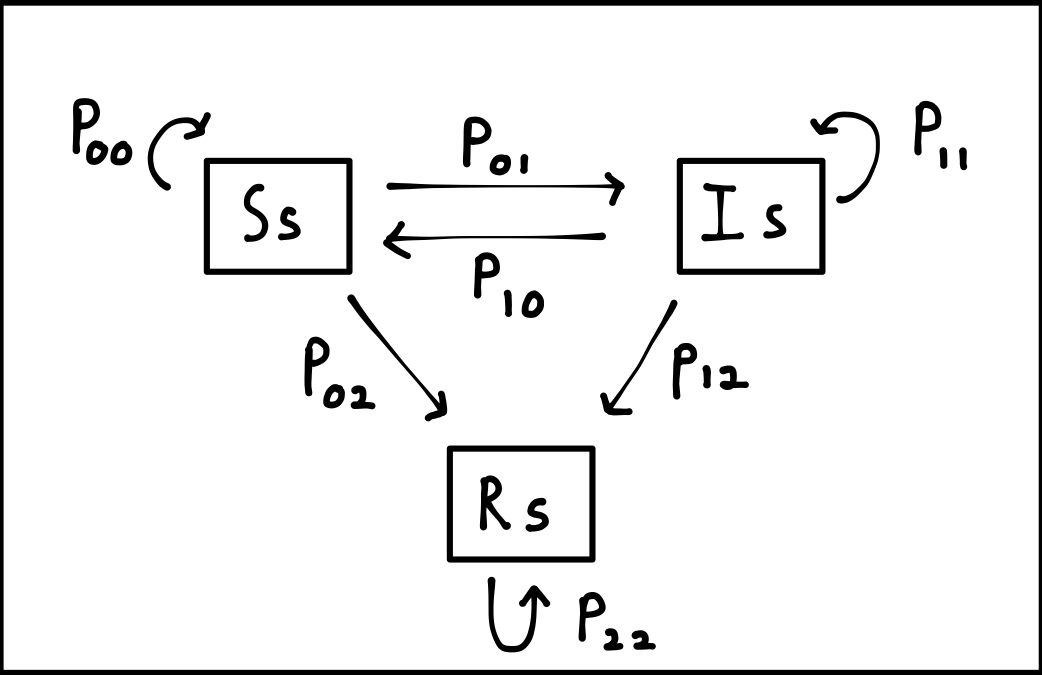
\includegraphics[width=10cm]{HepVisual.jpg}
    \caption{Hepatitis B Health States Visualized}
\end{figure} 

This results in the following Probability Matrix where $P_{ij}$ represents the transition property from State i to State j: 

\begin{equation*} 
P = 
    \begin{bmatrix}
    P_{00} & P_{10} & P_{20} \\
    P_{01} & P_{11} & P_{21} \\
    P_{02} & P_{12} & P_{22}
    \end{bmatrix}
=
    \begin{bmatrix}
    P_{00} & P_{10} & 0 \\
    P_{01} & P_{11} & 0 \\
    P_{02} & P_{12} & 1 \\
    
    \end{bmatrix}
\end{equation*}

\section{Data and Parameters}

Data on Hepatitis B patients was collected from a regional hospital in Ghana, an area with a very high prevalence rate of Hepatitis B.$^3$ From January 2016 to December 2016, Hepatitis B patients were monitored. The number of individuals and their corresponding health states after the 1 year time period are recorded here:
\\ \\

\begin{tabular}{ |p{2cm}||p{2cm}|p{2cm}|p{2cm}|p{2cm}|  }
 \hline
 \multicolumn{5}{|c|}{Number of Individuals in Hepatitis B Study} \\
 \hline
 Groups & Total & Susceptible State & Infected State & Removed State\\
 \hline
 Susceptible & 2929 &2281& 623 & 25\\
 \hline
 Infected & 623 & 0 &600 & 23\\
 \hline
\end{tabular}
\\
\\
\\
Using these values, the Transition Probability Matrix can be found by dividing the number of people who end up in a specific health state by the total number of people in the initial health state. For example:

\[ P_{01} = \frac{\text{Susceptible} \longrightarrow \text{Infected} }{\text{Initial Susceptible}} \ \ \textrm{= } \frac{623}{2929} \approx{0.21} \]
Since the Removed State is absorbing (does not transition into other states), the following probability matrix is formed: 

\begin{equation*}
P = 
\begin{bmatrix}
0.78 & 0 & 0 \\
0.21 & 0.96 & 0 \\
0.01 & 0.04 & 1
\end{bmatrix}
\end{equation*}
In order to predict probabilities in the long run, we need to use the Transition Matrix to calculate the steady state vector:

\begin{equation*}
P - I = 
\begin{bmatrix}
0.78 & 0 & 0 \\
0.21 & 0.96 & 0 \\
0.01 & 0.04 & 1
\end{bmatrix}
-
\begin{bmatrix}
1 & 0 & 0 \\
0 & 1 & 0 \\
0 & 0 & 1
\end{bmatrix}
=
\begin{bmatrix}
-0.22 & 0 & 0 \\
0.21 & -0.04 & 0 \\
0.01 & 0.04 & 0
\end{bmatrix}
\end{equation*}
To calculate the steady state vector, we need to calculate  ${x_1}, {x_2}, {x_3}$ by solving the following matrix equation:

\begin{equation*}
\begin{bmatrix}
-0.22 & 0 & 0 \\
0.21 & -0.04 & 0 \\
0.01 & 0.04 & 0
\end{bmatrix}
\begin{bmatrix}
x_1 \\
x_2 \\
x_3
\end{bmatrix}
= 0 
\end{equation*}
Solving the system of equations gives the following values:

\[
\systeme*{-0.22x_1 = 0, 0.21x_1 - 0.04x_2 = 0, 0.01x_1 + 0.04x_2 = 0}
\]

\begin{equation*}
x_1 = x_2 = 0
\end{equation*}
Since the probabilities of the Steady State Vector (S) must sum to 1, $x_3$ = 1:
\begin{equation*}
S =
\begin{bmatrix}
x_1 \\
x_2 \\
x_3
\end{bmatrix}
=
\begin{bmatrix}
0 \\
0 \\
1
\end{bmatrix}
\end{equation*}

\section{Benchmarking}

The Steady State Vector indicates that all individuals will transition into the absorbing Removed state in the long run. To test this, we can use the Transition Matrix to calculate probabilities for hypothetical Individuals X, Y, and Z.
\\ \\
\subsection{Individual X}
Patient X is currently in the Susceptible State with a 0.25 chance of transitioning into the Infected State and a 0.05 chance of transitioning into the Removed State. This individual's initial state is represented with the following vector:

\begin{equation*}
    X = 
    \begin{bmatrix}
   0.60 \\
   0.35 \\
   0.05
   \end{bmatrix}
\end{equation*}
To determine the probabilities for this individual in 10 years, we perform the following multiplication using the transition matrix and the initial state vector.  

\begin{equation*}
\text{After 10 Years}
\longrightarrow
   \begin{bmatrix}
    0.78 & 0 & 0 \\
    0.21 & 0.96 & 0 \\
    0.01 & 0.04 & 1
    \end{bmatrix} ^{10}
    \begin{bmatrix}
        0.60 \\
        0.35 \\
        0.05
   \end{bmatrix}
   =
   \begin{bmatrix}
        0.05 \\
        0.61 \\
        0.34
   \end{bmatrix}
\end{equation*}

\begin{figure}[htp]
    \centering
    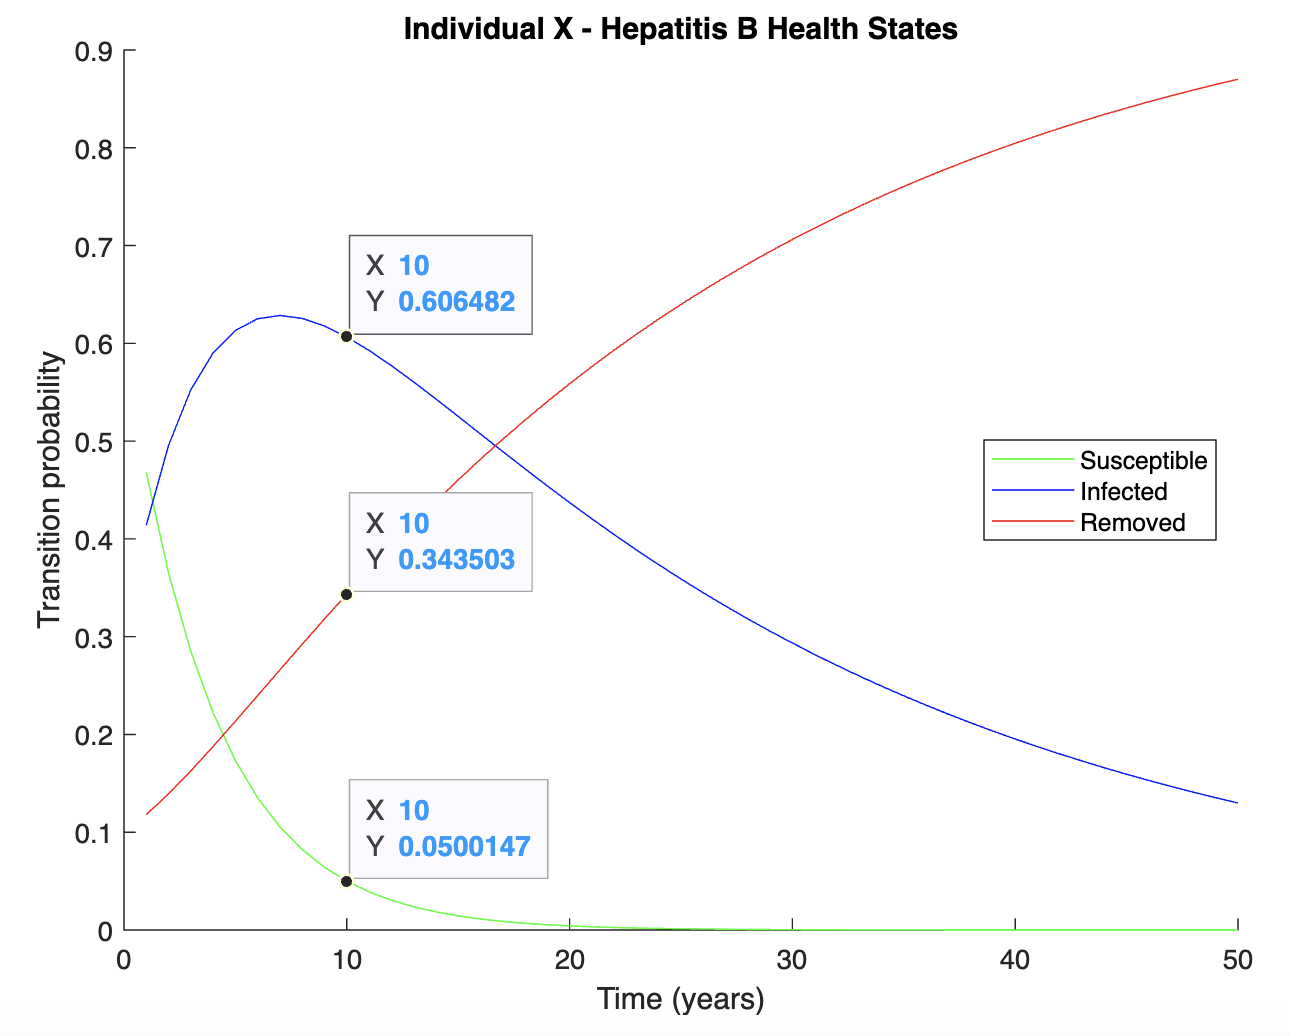
\includegraphics[width=14cm]{HepProbX.png}
    \caption{Hepatitis B Prediction Plot for Individual X}
\end{figure}

\newpage
\subsection{Individual Y}
Patient Y is currently in the Susceptible State with a 0.02 chance of transitioning into the infected state and a 0.01 chance of transitioning into the removed state.


\begin{equation*}
    Y = 
    \begin{bmatrix}
    0.97 \\
    0.02 \\
    0.01
   \end{bmatrix}
\end{equation*}
Multiply the transition matrix with the state vector Y:

\begin{equation*}
\text{After 10 Years}
\longrightarrow
   \begin{bmatrix}
    0.78 & 0 & 0 \\
    0.21 & 0.96 & 0 \\
    0.01 & 0.04 & 1
    \end{bmatrix} ^{10}
    \begin{bmatrix}
        0.97 \\
        0.02 \\
        0.01
   \end{bmatrix}
   =
   \begin{bmatrix}
        0.08 \\
        0.67 \\
        0.25
   \end{bmatrix}
\end{equation*}

\begin{figure}[htp]
    \centering
    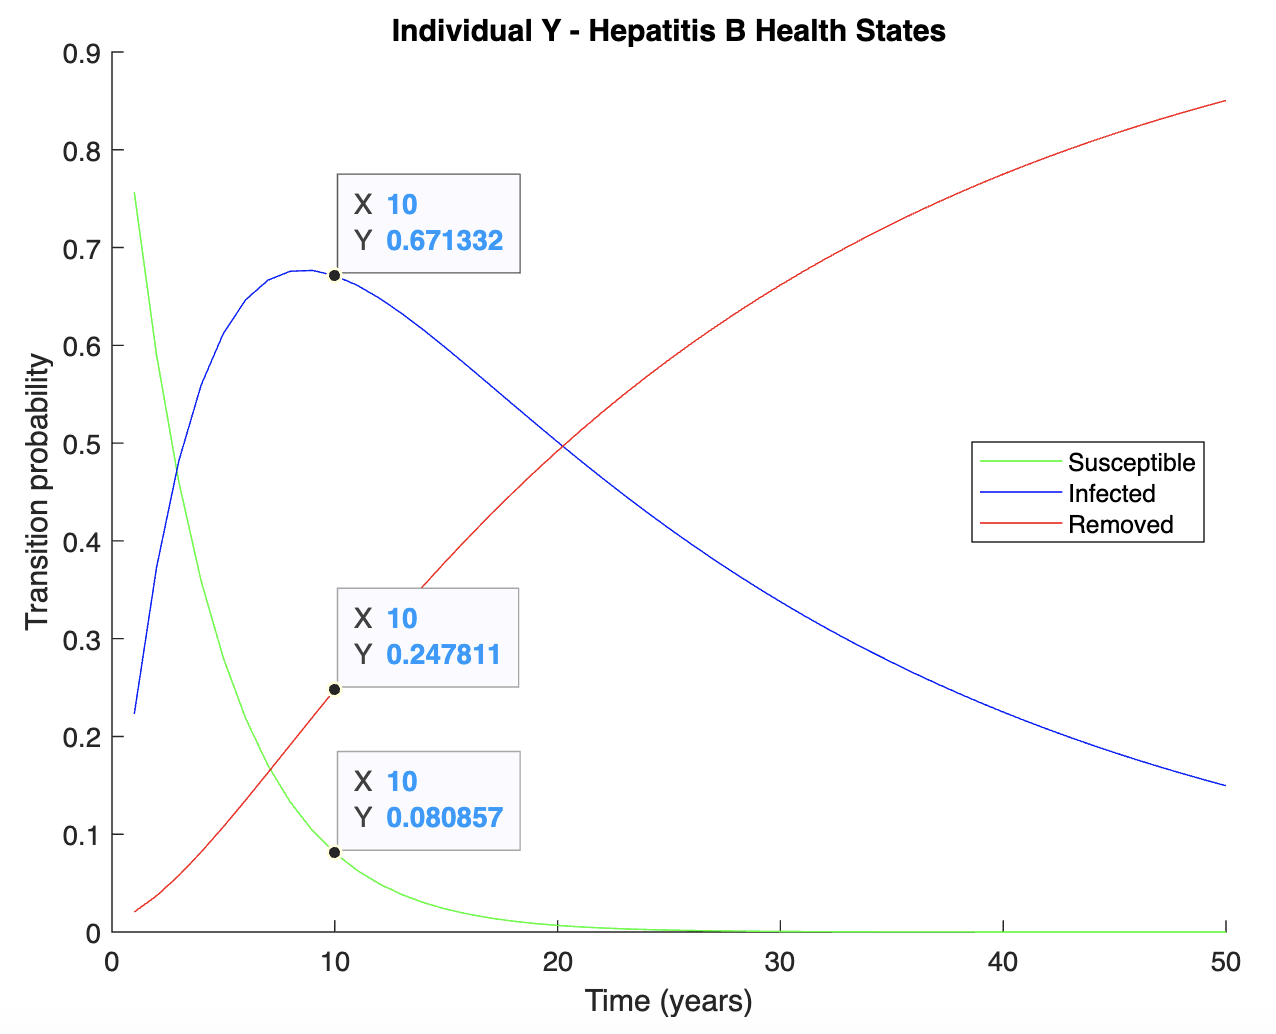
\includegraphics[width=14cm]{HepProbY.png}
    \caption{Hepatitis B Probabilities for Individual Y}
\end{figure}

\newpage
\subsection{Individual Z}
Patient Z is currently in the Infected State with a 0.01 chance of transitioning into the susceptible state and a 0.02 chance of transitioning into the removed state.

\begin{equation*}
    Z = 
    \begin{bmatrix}
    0.01 \\
    0.97 \\
    0.02
   \end{bmatrix}
\end{equation*}
Multiply the transition matrix with the state vector Z:

\begin{equation*}
\text{After 10 Years}
\longrightarrow
   \begin{bmatrix}
    0.78 & 0 & 0 \\
    0.21 & 0.96 & 0 \\
    0.01 & 0.04 & 1
    \end{bmatrix} ^{10}
    \begin{bmatrix}
        0.01 \\
        0.97 \\
        0.02
   \end{bmatrix}
   =
   \begin{bmatrix}
        0.00 \\
        0.65 \\
        0.35
   \end{bmatrix}
\end{equation*}

\begin{figure}[htp]
    \centering
    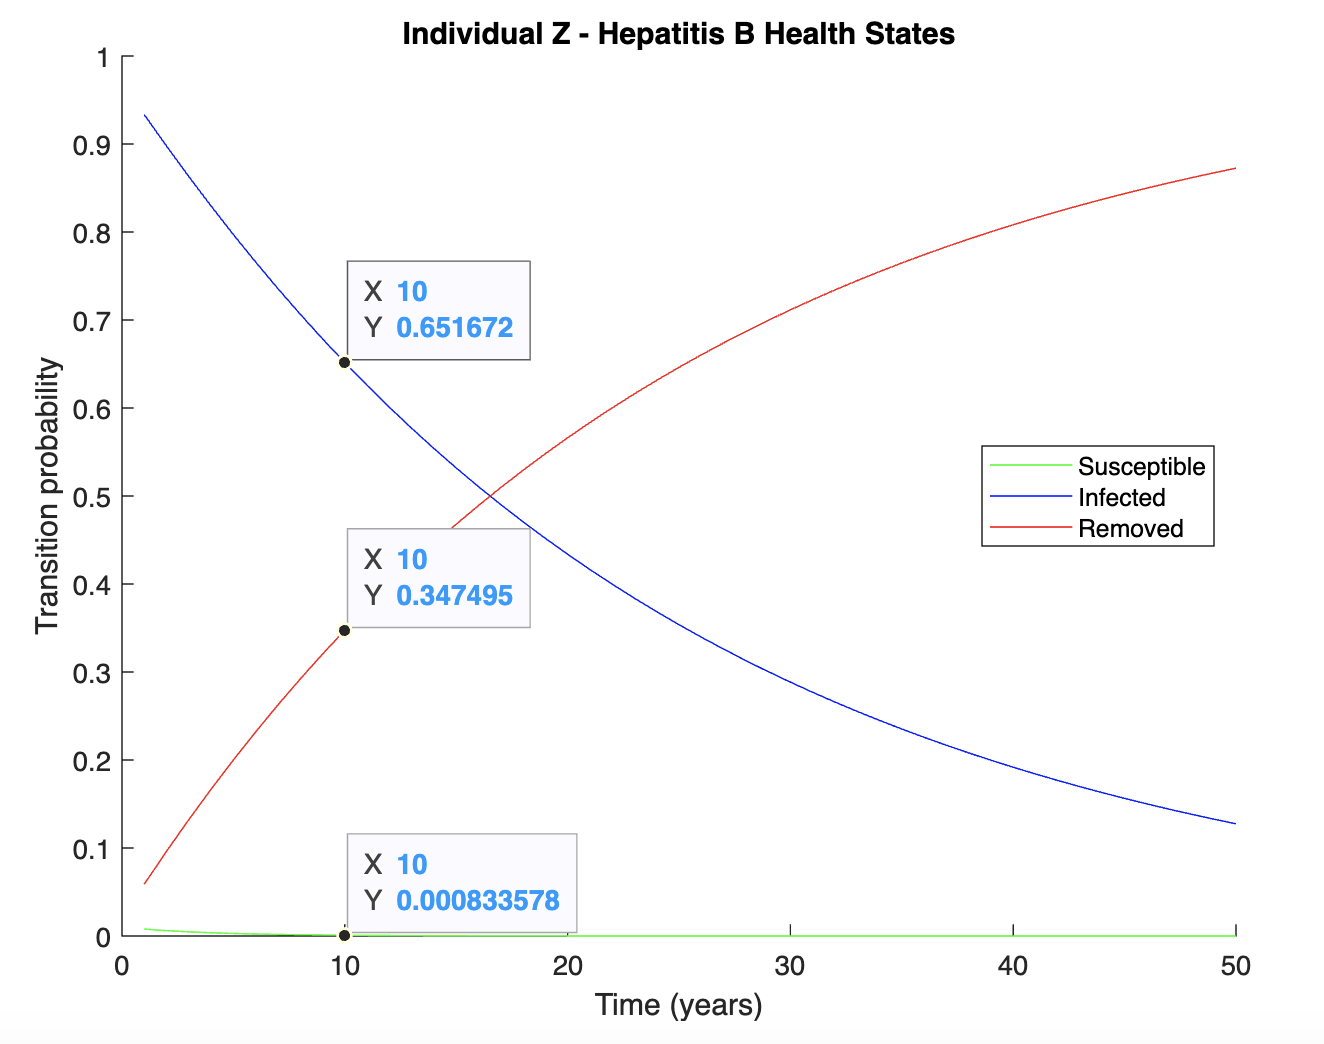
\includegraphics[width=14cm]{HepProbZ.png}
    \caption{Hepatitis B Prediction Plot for Individual Z}
\end{figure}

\newpage
\section{Results}

The transition probability matrix:

\begin{equation*}
P = 
\begin{bmatrix}
0.78 & 0 & 0 \\
0.21 & 0.96 & 0 \\
0.01 & 0.04 & 1
\end{bmatrix}
\end{equation*}
The Steady State Vector:
\begin{equation*}
S = 
\begin{bmatrix}
0 \\
0 \\
1
\end{bmatrix}
\end{equation*}
Using our Transition Matrix to predict health risks in 10 years for Individuals X, Y, and Z gives the following predictions:

\begin{equation*}
X_{10} = 
\begin{bmatrix}
        0.05 \\
        0.61 \\
        0.34
\end{bmatrix}
Y_{10} = 
\begin{bmatrix}
        0.08 \\
        0.67 \\
        0.25
\end{bmatrix}
Z_{10} = 
\begin{bmatrix}
        0.00 \\
        0.65 \\
        0.35
\end{bmatrix}
\end{equation*}
\\
These results reveal that after 10 years, Individuals X, Y, and Z will have a higher chance of transitioning into either the Infected State or the Removed State. Despite the differences in their initial health states, all three individuals become more prone to Hepatitis B as the calculated health state probabilities approach the Steady State Vector. Additionally, the graphs illustrate that in the long run the Susceptible and Infected probabilities will drop to 0 while the Removed probability becomes 1. 


\section{Discussion}

The Markov Model is able to predict the probabilities of an individual being in the three Hepatitis B health states (Susceptible, Infected, and Removed) after a certain amount of time. Using the Hepatitis B data collected from patients in Ghana, Transition Probability Matrix and the Steady State vector are calculated. Additionally, the absorbing Removed state is reflected in the Steady State vector since all individuals will transition into the removed state in the long run. 
\\ \\
To test the model, the health probabilities of 3 individuals are calculated by defining potential initial state vectors for each patient. Through benchmarking, it is revealed that the model is accurate because we expect individuals to become more vulnerable to the detrimental effects of Hepatitis B. As patients grow older, their immune system weakens and they become more likely to transition into the Removed state. To improve this model, we can consider age and gender when collecting patient data since Hepatitis B health risks will vary according to these factors. 

\newpage

\section{Matlab Code}
\lstinputlisting{Markov_HepB.m}

\section{Works Cited}
\begin{enumerate}
    \item https://www.cdc.gov/hepatitis/hbv/index.htm
    \item http://med.stanford.edu/liver/education/whatishepb.html
    \item https://www.hindawi.com/journals/ipid/2019/9362492/
\end{enumerate}

\end{document}
